\chapter{Approaches}\label{chapter:approaches}

\section{Key stroke pattern recognition}
Timings and patterns in key strokes individual characteristics, that can serve as biometric user identification. Individual typing patterns can be extracted from typing samples and can later be used to verify a users identity. The patterns, so called keystroke dynamics, are usually extracted via the key down / up events. Dholi and Chaudhari \cite{dholi2013typing} classified several features from those events, as shown in Figure~\ref{fig:keystrokeFeatures}: The interval between two key presses, the dwell time of a single key press, the latency between consecutive keystrokes, the flight time and the time from one up event to another.

\begin{figure}
    \centering
    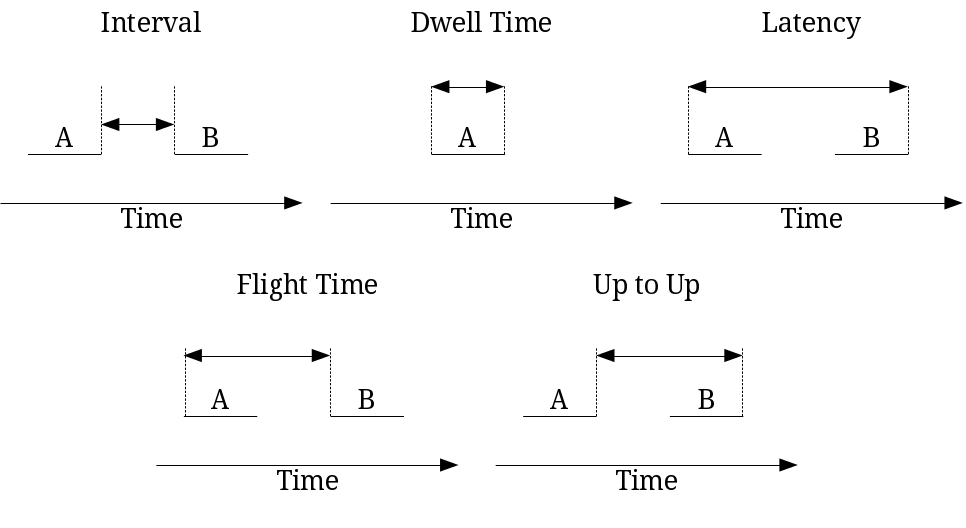
\includegraphics[width=\linewidth]{figures/KeystrokeTemporalFeatures.png}
    \caption{The five temporal features of keystroke dynamics\cite{dholi2013typing}}
    \label{fig:keystrokeFeatures}
\end{figure}
\subsection{Related work}
The idea of authentication by keystroke timings started as early as 1980 with Gaines \etal\cite{gaines1980authentication} to evaluate the effectiveness experimentally. In their experiment, the scientists gave seven professional typists, \ie secretaries, a text to type and examined their patterns in typing. Gaines \etal looked at the time to type pairs of successively typed letters, so called ``digraphs''. From five of these digraph times, all of the seven typists in this study could be identified.

In 1997, Dieter Bartmann presented PSYLOCK \cite{bartmann1997psylock}, a system that analyzes the keystroke rhythm of text input and identifies users according to these rhythms. The system claimes to work with an arbitrary text of aprox.\ 100 characters. PSYLOCK uses an approach based on statistical models in combination with support vector machines.

In 1999, Monrose and Rubin \cite{monrose2000keystroke} proposed a new approach at keystroke identification: Continuous keystroke verification. Previous attempts to keystroke verification only used static verification, \ie they verified the characteristics only at specific times, for example during login. Monrose's and Rubin's system monitors the user's typing behaviour continuously and thus can provide a significant improvement of security. The basic approach in their classification algorithm is clustering feature sets, determined through factor analysis, with a \gls{knn} approach.

Clarke and Furnell \cite{clarke2007authenticating} published a paper on identifying mobile phone users using keystroke analysis in 2006. In this paper, users were identified by typical handset interactions: entering telephone numbers and writing text messages.  Clarke and Furnell also compared several multi-layered neuronal networks of different flavour, all of which performed approximately the same. Since the form factor of mobile phones has drastically evolved in the last 10 years, their approach is largely obsolete for modern smartphones lacking physical buttons.
\subsection{Identification of keystrokes based on acceleration data}\label{subsection:keystrokerecognition}
Since smartphones lack physical buttons, but contain several high accuracy motion sensors, correlating taps on the screen with keystrokes seems not far fetched. Typical character input on phones is done via on-screen keyboards controlled via taps on the screen. 

With identifying keystroke patterns with acceleration sensor data, we are not limited to simple character and text input, but can also identify arbitrary tap sequences, that might occur in authentication scenarios. For example reading emails or messages is equally or even more secure-worthy than writing messages. Our approach can also extract and match patterns to authenticate users in simple navigation flow.

As a side note, typically the access to the on-screen keyboard is significantly restricted for \glspl{app} to hinder keyloggers from sniffing passwords. However, access to acceleration sensors is pretty much unrestricted and can also be done in web-browsers such as Google Chrome via an Javascript \gls{api} \cite{devicemotionjavascript}.

In 2012, Miluzzo \etal\cite{miluzzo2012tapprints} introduced \emph{TapPrints}, a mechanism to extract the location of screen taps solely from accelerometer and gyroscope data. With a machine learning approach, the system is able to detect taps with a bagged decision tree classifier to almost 100\%. Furthermore they were even able to guess individual letters in about 50\% of the cases.

For the scope of this bachelor's thesis, a complex training with machine learning algorithms to detect taps is unnecessary. We can detect individual taps via a simple peak detection algorithm, as described by Palishkar \etal\cite{palshikar2009simple}. An example for peak recognition on the time series of sensor measurements is shown in Figure~\ref{fig:peakdetection}, were ten peaks, corresponding to a ten tap sequence are detected. Eventual inaccuracies in identification of individual taps is not necessarily considered negative to the overall pattern recognition scheme, because those peaks are also part of the user's individual behaviour.

\begin{figure}
    \centering
    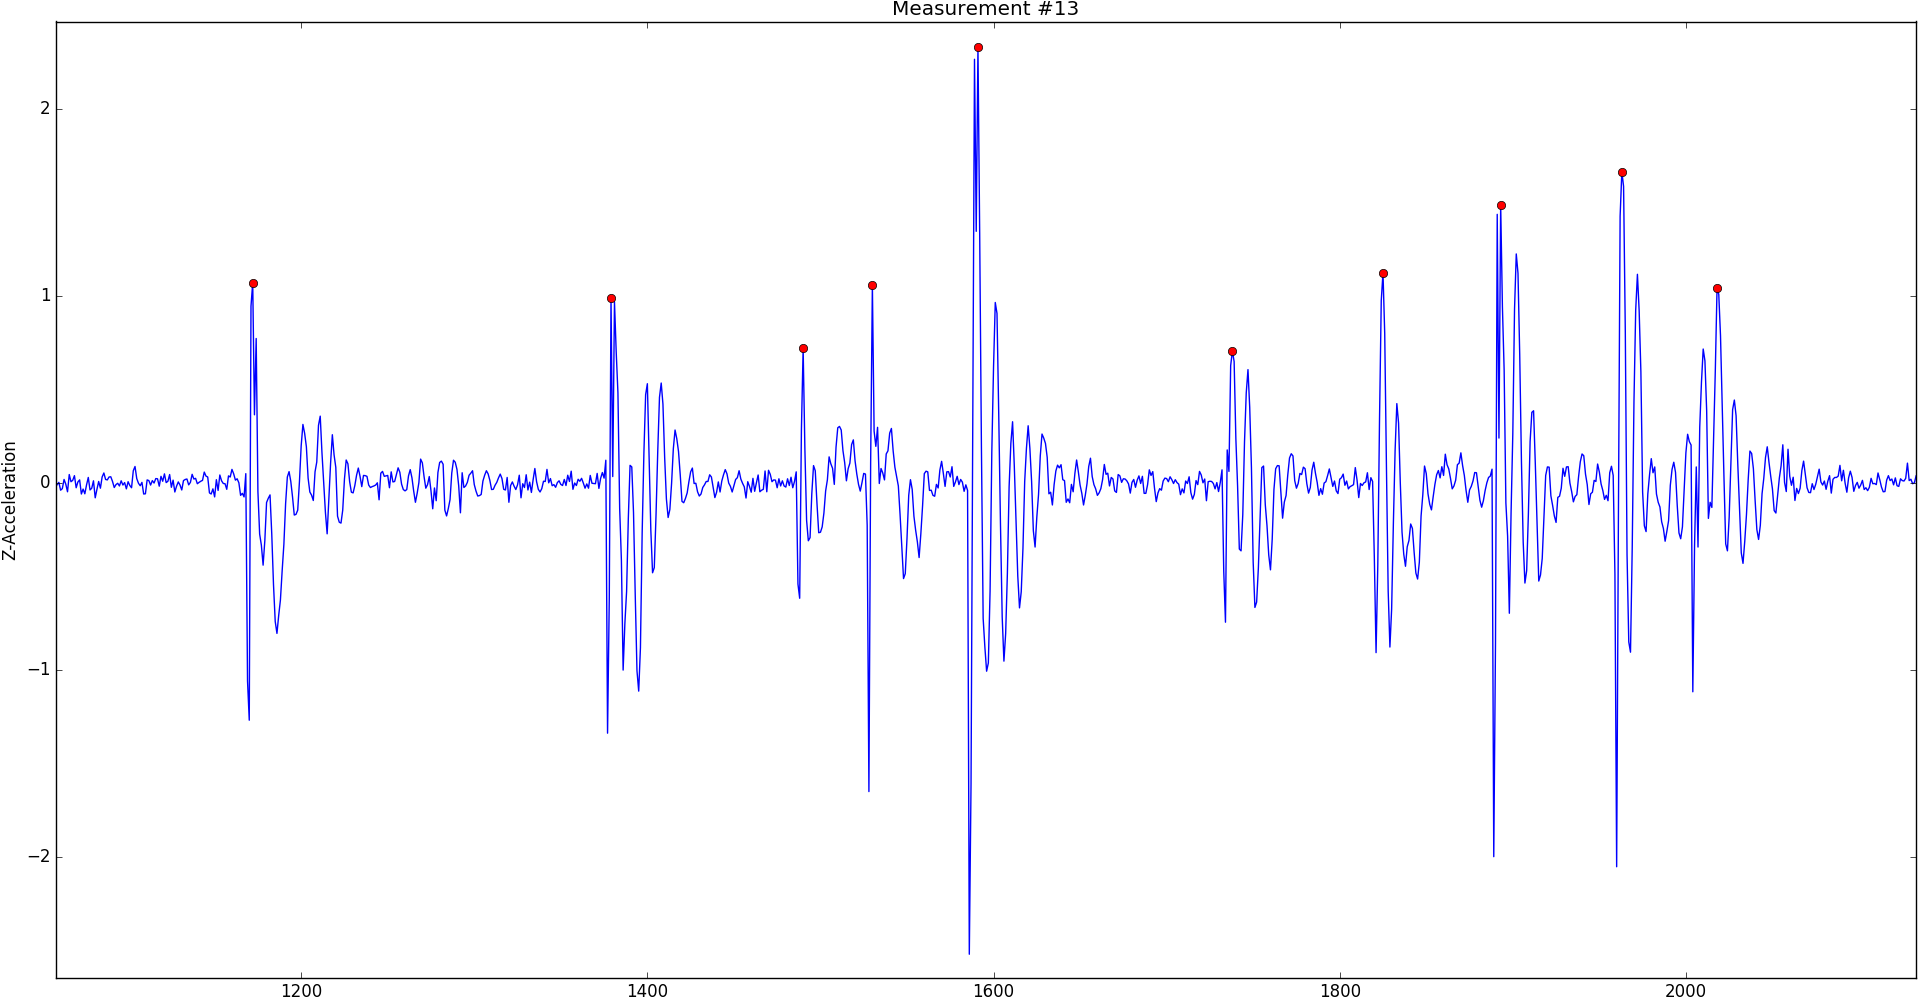
\includegraphics[width=\linewidth]{figures/detectedPeaks.png}
    \caption{Detected peaks in sensor measurements. Detected peaks are marked with red circles}
    \label{fig:peakdetection}
\end{figure}

Palishkar's peak detection algorithm identifies peaks (also called spikes) in a given time-series of values. These peaks represent keystrokes or simply ``values of interest'' in our acceleration data. Between the detected peaks, no disturbance in the phones acceleration is found, \ie the user did not touch or move the phone. A point in our data is a \emph{local} peak, if it is a maximum value within a defined window and not too many other points in the window have similar values.

Palishkar's algorithm is a parametric algorithm, that can be adapted to the individual structure of the time series data. The algorithm takes two parameters additional to the time series: the window size $k$ around the peak to detect and a stringency $h$ that rejects ``low'' peaks based on Chebyshev's inequality. Chebyshev's inequality states that for a random variable $X$ with mean $\mu$ and standard deviation $\sigma$: $P[|X - \mu| \geq h\sigma] < \frac{1}{h^2}$. Based on this inequality, we can make a sophisticated guess, that a peak $x$ with $|x - \mu| < (h * \sigma)$ is ``small'' in a global context and thus not a significant enough peak.

The window size $k$ restricts the amount of peaks detected within $k$ data points. To optimize the peak detection, we need to adapt $k$ to the typical time of a key press. Is $k$ too small, we might face the problem of detecting back-swings in the sensor data as additional peaks; is $k$ too big, subsequent keystrokes might not be recognized. We therefore analyzed typical usages to find a good $k$ in Section~\ref{subsection:featureextraction}.

\subsection{Features of keystrokes}
Historically, the features of key strokes were only extracted from the events keyboards reported to the operating system. In example the X.Org Server, the de-facto standard input handling system in UNIX-like operating systems, handles a single key press via two separate events: A \lstinline$KeyPress$ event, whenever a key is pressed down and a \lstinline$KeyRelease$ event, when the key is lifted up again.

These two events can now be measured in separate metrics, as shown in Figure~\ref{fig:keystrokeFeatures}. Furthermore, when considering more than two keystrokes, we can gather additional possible measurements:
\begin{itemize}
    \item Overall typing speed, usually measured in \gls{cpm}
    \item Overall typing rhythm and flow, measured in base frequencies
    \item Intensity of taps, measured by the amplitude of acceleration
\end{itemize}

These keystroke dynamics can be measured by several different aspects. To recognize typing patterns in arbitrary text, the typing patterns are usually broken down to di-graph, tri-graph of general $n$-graph segments. This means, that the overall typing pattern is reduced to sequences of $2, 3, ..., n$ key presses and only the features of these $n$-graphs are analyzed.

In our approach, we are monitoring the user's input in a controlled environment, \ie we only monitor input of the same sequence of characters, for example a password or a defined navigation sequence. This allows our approach to compare the whole sequence and we don't need to identify $n$--graphs in this user input. Extending our implementation to also extract these graphs might be a next step to improve the generality of the implementation in subsequent work.

\subsection{Adaption to phones}\label{subsection:phones}
For the implementation of keystroke recognition on smartphones, we first need to identify how to efficiently identify individual keystrokes. In this approach, we are considering text input directly on a smartphone with no additional devices, \ie the on-screen keyboard.
In Android, the inertial coordinate system for the acceleration sensors is as displayed in Figure~\ref{fig:deviceaxis}. The coordinate system, according to which the acceleration sensors report their measurements is defined relative to the default orientation of the device and are static, despite orientation changes of the devices display. The X-axis points horizontally to the right, the Y-axis vertically up and the Z-axis points towards the outside of the front face of the screen \cite{sensoreventandroidreference}.

\begin{figure}
    \centering
    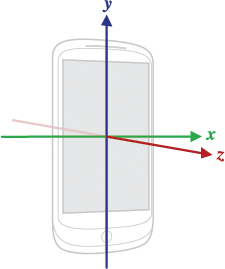
\includegraphics[width=0.5\textwidth]{figures/axis_device.png}
    \caption{Inertial coordinate system of Android devices \cite{sensoreventandroidreference}}
    \label{fig:deviceaxis}
\end{figure}

\begin{figure}
    \centering
    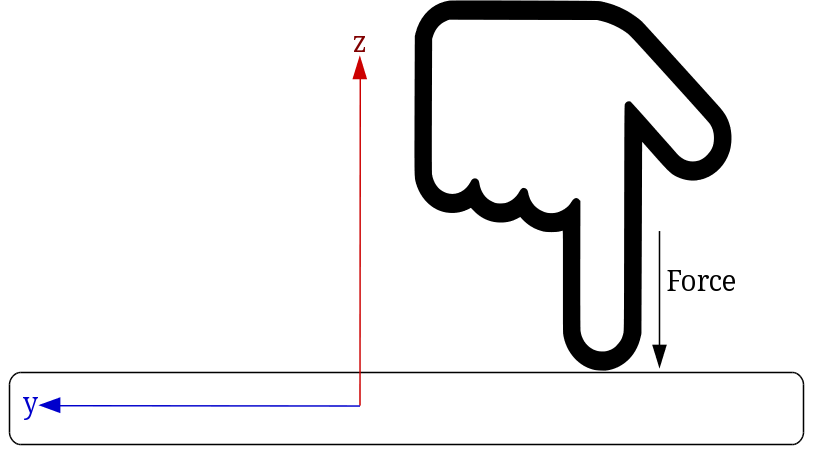
\includegraphics[width=\textwidth]{figures/TapDirection.png}
    \caption{Model of touches on Android devices}
    \label{fig:touchdirection}
\end{figure}
The main force of taps on a touchscreen is opposite to the direction of the Z-Axis as displayed in Figure~\ref{fig:touchdirection}. Thus, we can safely neglect the X- and Y-axis for our use-case of identifying individual taps on the screen.

The basic approach in keystroke classification on smartphones then would be to use a peak detection algorithm, as described in Section~\ref{subsection:keystrokerecognition}. We can apply this algorithm to the Z-axis acceleration sensor records of the phone, which yields sufficiently good data for individual taps.

\subsection{Adaption to watches and keyboards}
For recognition of key presses with smartwatches, we examined a scenario of a user wearing a smartwatch while typing on a physical keyboard. In this scenario, the X,Y-plane of the watch's inertial coordinate system is almost parallel to the keyboard (compare Figure~\ref{fig:watchcoordinate}).

\begin{figure}
    \centering
    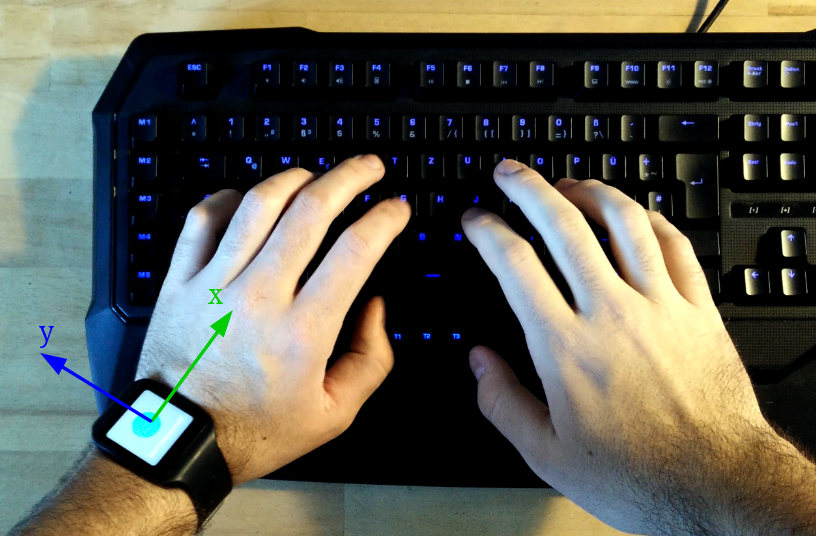
\includegraphics[width=0.9147\textwidth]{figures/WatchCoordinateSystem.png}
    \caption{The coordinate system of a smartwatch while typing on a keyboard}
    \label{fig:watchcoordinate}
\end{figure}

Wang \etal\cite{wang2015mole} discussed in their paper on MotionLeaks for MobiCom'15, that the key press timings on keyboards can be extracted by the Z-axis movement of the watch. When the user presses a key on the keyboard, the user's finger dips and the wrist also undergoes a partial dipping motion. This motion can be detected by the Z-axis acceleration, in combination with a peak detection algorithm, similar to the one used with phones in Section~\ref{subsection:phones}.

Wang \etal also improved their peak detection algorithm by chaining a peak detection tool with a bagged decision classifier. Since their goal was to guess individual typed keys instead of analysing the pattern as whole, the additional computational overhead might be worthwhile. This however, does not hold for our approach of matching the whole  input pattern, thus we use a simple peak detection algorithm.

Additionally to keystroke pattern recognition the overall movement of the watch while typing can be used as an additional authentication vector. Different users might move their hands differently for text input. However we are not aware of scientific studies measuring the effectiveness of this approach.

\section{Gait recognition}
Gait is defined as ``the way in which a person (\ldots) walks'' in the Cambridge Dictionary. Various scientific papers analyzed the specifics of human gait \cite{johansson1975visual, lee2002gait, johnstonsmartwatch} and concluded, that individual gait can be used as a biometrical recognition mechanism. The steps a user walks throughout the day can for example be used to generate user profiles and extract an identifying pattern. 

As early as 1975, Johansson \cite{johansson1975visual} has shown, that observers could identify individuals just by watching videos of lights mounted to joints of otherwise invisible walking people. Additionally, the observers were able to not only identify previously known people, but also identify the gender of unknown persons. However human gait is influenced by many more personal aspects, as the individual weight, leg length, posture and speed of walking. Thus gait patterns are highly individual and are usually unique.
\subsection{Related work}
The early attempts to gait recognition used video footage and moving light displays to extract the gait information. This approach works quite well, but is largely unpractical since face and shape recognition algorithms work even more precise on videos. Starting in 2005 with Mäntyjärvi \etal\cite{mantyjarvi2005identifying}, researchers used accelerometers to extract gait information of users. These sensors were attached to different body parts, such as hip, arms and feet to evaluate the recordable data. Optimal positioning of these accelerometers is still disputed, but recent studies showed, that portable devices such as commercial phones \cite{derawi2013gait} or smartwatches \cite{johnstonsmartwatch} are sufficiently good sensors for gait recognition.

For gait recognition with mobile phones, Schmidtbartel \cite{thesisschmidbartl} implemented a framework to recognise specific user-device combinations. His model accumulated sensor data of the user's gait and aggregates a median step pattern, as shown in Figure~\ref{fig:gaitacceleration}. 
\begin{figure}
    \centering
    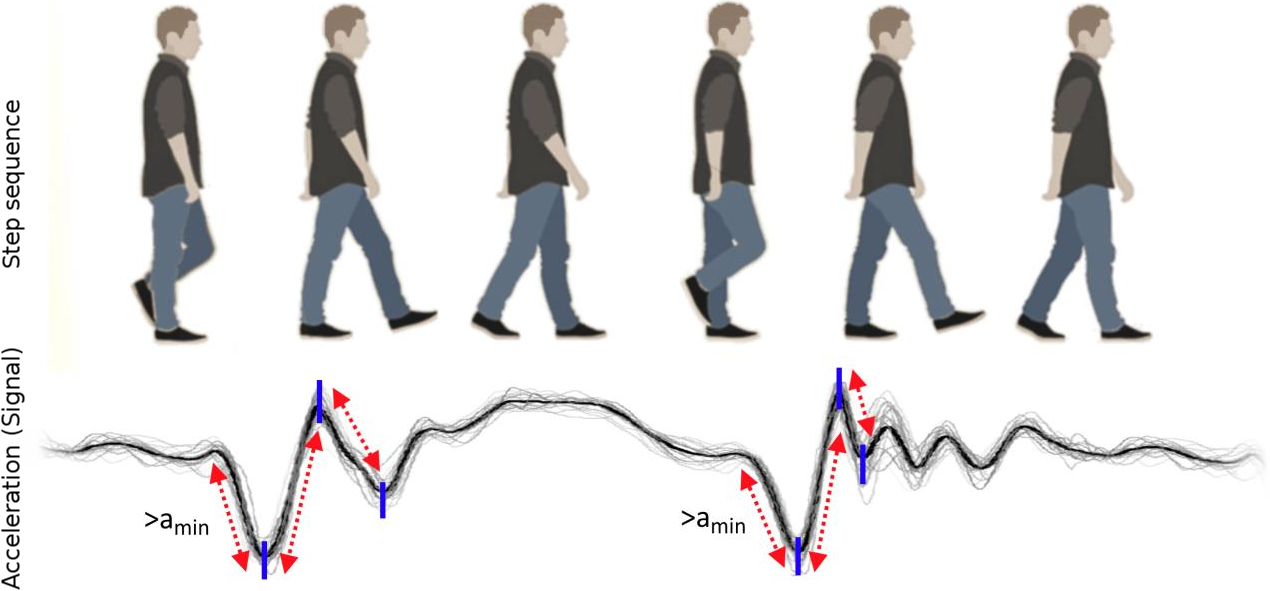
\includegraphics[width=\textwidth]{figures/GaitAcceleration.png}
    \caption{Motion circle and corresponding measured acceleration data \cite{thesisschmidbartl}}
    \label{fig:gaitacceleration}
\end{figure}

Each individual recorded step circle may vary due to signal noise or different user behaviour. Shown in the bottom half of the figure as individual lines, individual step circles are recorded in light grey. In black, the calculated median is shown. To calculate this value, multiple steps are clustered, according to the similarity of those steps. As a result, there might be multiple clusters of gait signals, \ie for walking, jogging or running.

Schmidtbartel is using an \gls{manhattandistance} metric in his implementation, however other researchers \cite{derawi2013gait} suggest, that \gls{dtw} and an extension of \gls{dtw}, called Cross \gls{dtw} Metric even result in better gait recognition performance.

\subsection{General limitations}
To monitor the gait patterns of users, constant monitoring of the devices sensors is necessary, even though the user is not actively using the device. This prevents the device to go in so called ``deep sleep'' state where less energy is consumed. Since battery is mostly a big concern on mobile devices, this is a major deal-breaker. Users tend to deinstall battery draining applications quickly.

For authentication purposes, an timely response to whether or not the authentication attempt was successfully is required. However, gait is not available all the time and certainly not on demand. Prompting the user to take a walk to get access to his data is not an option.

\subsection{Conclusion}
As consequence of these limitations, we decided against using an gait recognition approach as personal authentication factor. Nonetheless, gait recognition might be an additional approach for intrusion detection. For example the device itself can recognise it being stolen by detecting other gait patterns. This allows the device to take counter-measures, \eg lock itself, alert the user and activate ``Find My Device'' functionality.
In contrast, gait recognition is not suitable for concrete, immediate authentication needs, as it is the vision of this thesis.